%% RiSE Latex Template - version 0.5
%%
%% RiSE's latex template for thesis and dissertations
%% http://risetemplate.sourceforge.net
%%
%% (c) 2012 Yguaratã Cerqueira Cavalcanti (yguarata@gmail.com)
%%          Vinicius Cardoso Garcia (vcg@cin.ufpe.br)
%%
%% This document was initially based on UFPEThesis template, from Paulo Gustavo
%% S. Fonseca.
%%
%% ACKNOWLEDGEMENTS
%%
%% We would like to thanks the RiSE's researchers community, the 
%% students from Federal University of Pernambuco, and other users that have
%% been contributing to this projects with comments and patches.
%%
%% GENERAL INSTRUCTIONS
%%
%% We strongly recommend you to compile your documents using pdflatex command.
%% It is also recommend use the texlipse plugin for Eclipse to edit your documents.
%%
%% Options for \documentclass command:
%%         * Idiom
%%           pt   - Portguese (default)
%%           en   - English
%%
%%         * Text type
%%           bsc  - B.Sc. Thesis
%%           msc  - M.Sc. Thesis (default)
%%           qual - PHD qualification (not tested yet)
%%           prop - PHD proposal (not tested yet)
%%           phd  - PHD thesis
%%
%%         * Media
%%           scr  - to eletronic version (PDF) / see the users guide
%%
%%         * Pagination
%%           oneside - unique face press
%%           twoside - two faces press
%%
%%		   * Line spacing
%%           singlespacing  - the same as using \linespread{1}
%%           onehalfspacing - the same as using \linespread{1.3}
%%           doublespacing  - the same as using \linespread{1.6}
%%
%% Reference commands. Use the following commands to make references in your
%% text:
%%          \figref  -- for Figure reference
%%          \tabref  -- for Table reference
%%          \eqnref  -- for equation reference
%%          \chapref -- for chapter reference
%%          \secref  -- for section reference
%%          \appref  -- for appendix reference
%%          \axiref  -- for axiom reference
%%          \conjref -- for conjecture reference
%%          \defref  -- for definition reference
%%          \lemref  -- for lemma reference
%%          \theoref -- for theorem reference
%%          \corref  -- for corollary reference
%%          \propref -- for proprosition reference
%%          \pgref   -- for page reference
%%
%%          Example: See \chapref{chap:introduction}. It will produce 
%%                   'See Chapter 1', in case of English language.
%%
%% Citation commands:
%%          \citet (from natbib) -- To cite a reference as part of the narrative
%%          \citep (from natbib) -- To cite a reference between parenthesis
%%          citationblock environment -- To produce direct citation blocks according to the ABNT

\documentclass[en,oneside,onehalfspacing,bsc]{risethesis}
\usepackage{colortbl}
\usepackage{color}
\usepackage[table,xcdraw]{xcolor}
\usepackage{longtable}
\usepackage{microtype}
\usepackage{bibentry}
\usepackage{subfigure}
\usepackage{multirow}
\usepackage{multicol}
\usepackage{rotating}
\usepackage{booktabs}
\usepackage{pdfpages}
\usepackage{caption}
\usepackage{lipsum}
\usepackage{sectsty}

\usepackage{tikz}
\usetikzlibrary{calc,trees,positioning,arrows,chains,shapes.geometric,%
    decorations.pathreplacing,decorations.pathmorphing,shapes,%
    matrix,shapes.symbols}
\tikzset{
>=stealth',
  punktchain/.style={
    rectangle, 
    rounded corners, 
    % fill=black!10,
    draw=black, very thick,
    text width=7em, 
    minimum height=3em, 
    text centered, 
    on chain},
  line/.style={draw, thick, <-},
  element/.style={
    tape,
    top color=white,
    bottom color=blue!50!black!60!,
    minimum width=8em,
    draw=blue!40!black!90, very thick,
    text width=10em, 
    minimum height=3.5em, 
    text centered, 
    on chain},
  every join/.style={->, thick,shorten >=1pt},
  decoration={brace},
  tuborg/.style={decorate},
  tubnode/.style={midway, right=2pt},
}

\captionsetup[table]{position=top,justification=centering,width=.85\textwidth,labelfont=bf,font=footnotesize}
\captionsetup[lstlisting]{position=top,justification=centering,width=.85\textwidth,labelfont=bf,font=footnotesize}
\captionsetup[figure]{position=bottom,justification=centering,width=.85\textwidth,labelfont=bf,font=footnotesize}

%% Chapter and (Sub)Section fonts must be same size as text (12)
\sectionfont{\fontsize{12}{15}\selectfont}
\subsectionfont{\fontsize{12}{15}\selectfont}
\subsubsectionfont{\fontsize{12}{15}\selectfont}

%% Change the following pdf author attribute name to your name.
\usepackage[linkcolor=black,
            citecolor=black,
            urlcolor=black,
            colorlinks,
            pdfpagelabels,
            pdftitle={Rise Thesis Template (ABNT)},
            pdfauthor={Rise Thesis Template (ABNT)},
            breaklinks=true]{hyperref}

\address{RECIFE}

\universitypt{Universidade Federal de Pernambuco}
\universityen{Federal University of Pernambuco}

\departmentpt{Centro de Informática}
\departmenten{Center for Informatics}

\programpt{Graduação em Engenharia da computaç}
\programen{Undergraduate in Computer Engineering}

\majorfieldpt{Engenharia da computação}
\majorfielden{Computer Engineering}

\title{Evaluation of Machine Learning Algorithms in the Categorization of Android API Methods into Sources and Sinks}

\date{2018}

\author{Walber de Macedo Rodrigues}
\adviser{George Darmiton da Cunha Cavalcanti}

% Macros (defines your own macros here, if needed)
\def\x{\checkmark}

\begin{document}

\frontmatter

\frontpage

%\presentationpage

%\begin{fichacatalografica}
%	\FakeFichaCatalografica % Comment this line when you have the correct file
%     \includepdf{fig_ficha_catalografica.pdf} % Uncomment this
%\end{fichacatalografica}

%\banca

%\begin{dedicatory}
%I dedicate this thesis to all my family, friends and professors who gave me the
%necessary support to get here.
%\end{dedicatory}

%\acknowledgements
%\input{agradecimentos}

%\begin{epigraph}[]{Poul Anderson}
%I have yet to see any problem, however complicated, which, when looked at in the
%right way, did not become still more complicated.
%\end{epigraph}

\let\cleardoublepage\clearpage

\resumo
% Escreva seu resumo no arquivo resumo.tex
{\parindent0pt
	Um programa computa em dados sensíveis e não sensíveis, esses dados seguem um fluxo específico indo de \textit{data sources} para \textit{data sinks}. O vazamento de dados acontece quando dados sensíveis chegam sem autorização em \textit{sinks}, para prevenir isso,  técnicas estáticas e dinâmicas de \textit{Flow Enforcement} garantem que esses dados não cheguem nessas \textit{sinks}. Para isso, esses métodos usam listas, geradas manualmente, de métodos que sejam \textit{sources} sensíveis ou \textit{sinks}, e essa solução é impraticável para grandes APIs como a do Android. Visto isso, uma abordagem usando \textit{machine learning} foi desenvolvida para classificar esses métodos \textit{sources} e \textit{sinks}. \\

O presente trabalho tem como objetivo criar um dataset para avaliar os métodos de classificação Monolítios e Sistemas Multiclassificadores para decidir qual é o mais apropriado para esse problema. Para criar o dataset, foram utilizados as APIs Android Level 3 a Level 27, excluindo as de Level 18 e 20, abrangendo a maioria das APIs recentes que foram aplicadas em um extrator de features. Para realizar a classificação, foram amostrados aleatoriamente 30 datasets de treino e teste, foram avaliados precisão, recall, F1 score e acurácia dos classificadores em cada um dos datasets e feito um teste de hipótese. Neste trabalho concluimos que o MLP tem melhores resultados no problema de classificação de métodos Android, METADES com árvore de decisão e SVM também tem um resultado satisfatório e ficam estatisticamente empatados com o MLP.

}

\abstract
% Write your abstract in a file called abstract.tex
{\parindent0pt
	A program computes in either sensitive and non-sensitive data and follows a specific flow, from data sources to data sinks.
Data leakage happens when sensitive data is sent to unauthorized data sinks, to prevent that, Dynamic and Static Flow Enforcement 
techniques ensure that sensitive data reaches those sinks. To prevent data leakage, 
these methods rely on a list of sensitive data sources and data sinks, this list is hand annotated and is impractical to be made to a huge API such as Android. 
With that in mind, a machine learning model is used to classify methods into sources and sinks. 
The present work intends to extend the previous work creating a dataset to evaluate the most used classification algorithms and define which is the most suitable to this problem.
}

% List of figures
\listoffigures

% List of tables
\listoftables

% List of acronyms
% Acronyms manual: http://linorg.usp.br/CTAN/macros/latex/contrib/acronym/acronym.pdf
\listofacronyms
\begin{acronym}[ACRONYM] 
% Change the word ACRONYM above to change the acronym column width.
% The column width is equals to the width of the word that you put.
% Read the manual about acronym package for more examples:
%   http://linorg.usp.br/CTAN/macros/latex/contrib/acronym/acronym.pdf

\end{acronym}

% Summary (tables of contents)
\tableofcontents

\mainmatter

% Uncomment to graduation
\chapter{Introduction}

\section{Motivation}

The expression Internet of Things is relatively new, was coined between 1997 and 2000 and consist of devices that sense or actuate in a real environment (\cite{minerva2015towards}). The number of IoT devices has already overcame the living humans on Earth and, by 2020, is estimated to exist about 20 billion of IoT devices connected to the internet \citep{iotmarket}. It is very common that these devices have a companion app, cloud or mobile based which are used to control and monitor the IoT devices.

This growing popularity come along with major security and privacy issues, hackers are exploiting Android apps to leak user private information or hijacking the IoT device to use in other attacks, such as DDoS \citep{ycraig}. The information leak is very concerning from a privacy point of view, as a vast majority of user sensitive information is stored in smartphones, GPS location, text messages, photos and even bank data can be stolen if exists an issue in IoT companion apps.

IoT applications consists in a device that can sense and actuate in the real environment which is controlled and monitored using mobile apps or a web server to serve for any kind of purpose, from medical monitoring to smart wearable devices. Depending of the application the devices are designed to last for years with low or no need of maintenance or be portable. To ensure that these devices are hardware constrained, lacking computational power to ensure a longer battery life \citep{raj2017internet}. This leads to some issues: the needing of newer lightweight security protocols to fit the hardware constrains as \cite{zhang2014iot} points and a reduced set of communications protocols and interfaces to keep low power consumption.

The lack of communications protocols forced the industry to create other devices to act as an IoT hub, if the IoT does not have an independent connection to the internet, hub architectures are common if the device have simpler and short communication protocols, like Bluetooth, RFID, ZigBee and NFC \cite{al2017internet}. The hub concentrate the communications between the devices and the companion app, this app is a mobile or cloud application that provides monitoring and control for the IoT devices. The real IoT communication architecture is very diverse but a device have few options, it can only send information through the hub to the cloud, to a smartphone, directly to the cloud or have these three combined using a mixed architecture.

In Figure \ref{fig:arch-direct} we can observe how the IoT device communicate directly to user devices, the smart devices are represented by a smart bulb and the user devices by a smartphone and a desktop computer. The full arrows express that that the link must exist to have a connection. In Figure \ref{fig:arch-hub}, we have a intermediate device that makes the connection between the device and the user, the hub can aggregate as many IoT devices as intended. The cloud architecture Figure \ref{fig:arch-cloud} consists in a device that is connected to the internet using a router, which sends and receives user actions using the cloud as intermediary. The mixed architecture, Figure \ref{fig:arch-mixed}, can have all the previous kind of connections, the user has freedom to send information directly to the device, or use a hub to control the devices with only one application or send remote requests using any cloud provider.

\begin{figure}[ht] 
    \begin{minipage}[b]{0.5\linewidth}
        \centering
        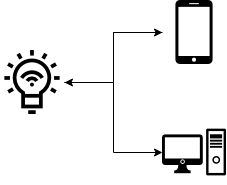
\includegraphics[width=0.6\linewidth]{images/iot-architectures/direct.png}
        \caption{Direct architecture}\label{fig:arch-direct}
        \vspace{4ex}
    \end{minipage}%%
    \begin{minipage}[b]{0.5\linewidth}
        \centering
        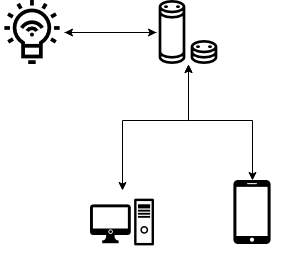
\includegraphics[width=0.6\linewidth]{images/iot-architectures/hub.png}
        \caption{Hub architecture}\label{fig:arch-hub}
        \vspace{4ex}
    \end{minipage} 
    \begin{minipage}[b]{0.5\linewidth}
        \centering
        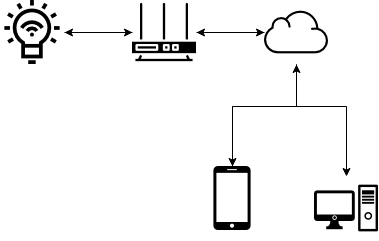
\includegraphics[width=0.8\linewidth]{images/iot-architectures/cloud.png}
        \caption{Cloud based architecture}\label{fig:arch-cloud}
        \vspace{4ex}
    \end{minipage}%% 
    \begin{minipage}[b]{0.5\linewidth}
        \centering
        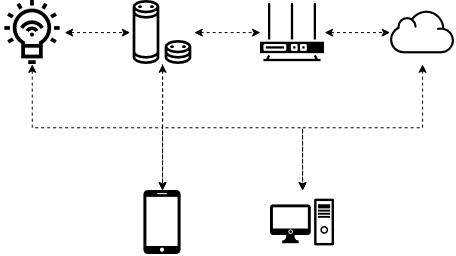
\includegraphics[width=1\linewidth]{images/iot-architectures/mixed.png}
        \caption{Mixed architecture}\label{fig:arch-mixed}
        \vspace{4ex}
    \end{minipage} 
\end{figure}

With the increasing popularity of IoT, attackers are exploiting weakness in the architecture, the device itself and the smartphones that hosts the application. Exists many known attacks, from leaking user data as described by \cite{ycraig} to hijacking the device to use in other attacks such as DDoS using botnets \citep{kolias2017ddos}. The information leaking is a major concern from a privacy point of view, this kind of attack can leak any kind of user sensitive data being sent to malicious hosts or unaware to a cloud server. 

Sensitive data is any data that can be used to identify the user or any private user information, such as photos, International Mobile Equipment Identity (IMEI), biometric data, GPS localization, bank information and private messages. Non-sensitive data is any dynamic information that do not identify the user, often, this kind of information if public or shared, such as application source code.

Every program computes on either sensitive data or non-sensitive data, and this data follows a specific flow, first it is acquired from data sources and sent to data sinks \citep{mccabe2003network}. Data sources, in the context of mobile and IoT devices, are defined as method calls that read data from shared resources such as phone calls, screenshots, sensor polling data from ambient, device identification numbers \citep{rasthofer2014machine}. Data sinks are methods calls that have at least one argument, this argument is non-constant data from the source code \citep{rasthofer2014machine}. The data sink can be an interface to the user or system API for communication to other devices or store data \citep{viet2010specifying}.

To address the data privacy issue, mobile operating systems such as Android and IOs have a permission based system intended to control which sensitive information the application have access, like contact numbers, photos, videos and data from camera and microphone. These permissions are granted by the user at the installation or during the application usage (\cite{androidpermissions}). An issue existing in the permission system is called superprivileges, where the apps asks for unnecessary permissions, caused by developers that misunderstanding the API (\cite{felt2011android}). There is a methodology that help the developers to have a broader knowledge of the permissions in Android that has been proposed by \cite{barrera2010methodology}.

Another issue created when using the permission system is the abuse of privilege given by the user to an app, or even, the application can intentionally send information to a malicious host. As \cite{jiang2012dissecting} reports, there are malwares that are capable to steal sensitive information from the user, like SMS. To solve unwanted sensitive information flow inside Android applications, \cite{arzt2014flowdroid}, \cite{wei2014amandroid} and \cite{gordon2015information} developed static and dynamic ways to enforce that this kind of information does not leak to unwanted sink methods. The dynamic way to enforce information flow is called Dyanmic Flow Enforcement and statically is called Static Flow Enforcement. These methods are going to be presented in a deeper fashion in Chapter \ref{chapter:background}.


\section{Objective}\label{section:background}

This work has two main objectives: generate a public database containing methods from Android APIs and evaluate the performance of the state of the art classification algorithms on this database. The methods should be classified into source or sink of sensitive information, or neithernor.

The motivation behind the database creation comes when \cite{rasthofer2014machine} developed the initial classification work. Their objective were create a machine-learning solution to identify sources and sink methods from the code of any Android API. So, every time that you wanted to test other classification algorithms, you had to extract the methods and features if you evaluate in other API. This implies in extracting the API from a real Android device, which can be tricky if the person does not have this specific knowledge. Then, create a public database extract knowledge and develop better solutions to this problem is very likely.

The objective of evaluate different classification algorithms comes as \cite{rasthofer2014machine} shows results  for only three classification algorithms, SVM, Decision Tree and Naive Bayes. From that, emerged the question if other classification algorithms have better results in this database. So, the second objective is to evaluate the most used classifiers in the literature, SVM, Naive Bayes, Decision Trees, MLP, KNN, including ensemble classifications methods.


\section{Work Structure}\label{section:structure}

This work is divided as follows: Chapter \ref{chapter:background} is a short introduction about Static and Dynamic Analysis, followed by a explanation about Flow Enforcement techniques, which is important to understand what issues these methods addresses and what are the limitations. In Chapter \ref{chapter:architecture} we introduce the methodology used in this work and the training and test architectures used by the machine learning methods. Chapter \ref{chapter:results} we show the results archived, the dataset created and the scores of each classifier used in this work and we report our conclusions in Chapter \ref{chapter:conclusion}.

\chapter{Background}\label{background}
\chapter{Machine Learning Models}

\section{Monolithic}
    \subsection{Decision Tree}\label{decisiontree_section}
    \subsection{K-Nearest Neighbors}\label{knn_section}
    \subsection{Multi Layer Perceptron}\label{mlp_section}
    \subsection{Naive Bayes}\label{naive_bayes_section}

    \subsection{Random Forests}\label{rf_section}

    \subsection{Support Vector Machine}\label{svm_section}

\section{Dynamic Classifier Selection}
    \subsection{KNORAE}\label{knorae_section}
    \subsection{KNORAU}\label{knorau_section}
    \subsection{META-DES}\label{metades_section}
    \subsection{OLA}\label{ola_section}
    \subsection{Single Best}\label{sb_section}
    \subsection{Static Selection}\label{ss_section}
\chapter{Architecture}\label{chapter:architecture}

The proposed architecture consists in two steps, a training step and test step: the training step is shown in Figure \ref{figure:train-flow} and the test tep is shown in Figure \ref{figure:test-flow}. The training step consists in extract features from real Android methods and use that combined with the real classes to train classifiers. The first step to create the classifiers to is to have a list of fully implemented Android APIs and a list of already classified methods.

The APIs used in this work have been selected from two different repositories: the default repository of Android images used by \cite{rasthofer2014machine} and the second repository is a well known set of Android images, provided by \cite{hiddenapi}, which is used by mobile developers that need methods available only in fully implemented APIs, that are only available when the API is extracted from real devices. The APIs from level 3 to 17 used in this work were extracted from \cite{rasthofer2014api} and the APIs 17, 19 and 21 to 27 gathered from \cite{hiddenapi}. These two APIs repositories meet the requirement imposed by \cite{rasthofer2014machine}, and consists that the APIs used need to have the fully method implementation, done by extracting APIs from real devices.

\begin{figure}[!h]
    \begin{center}
        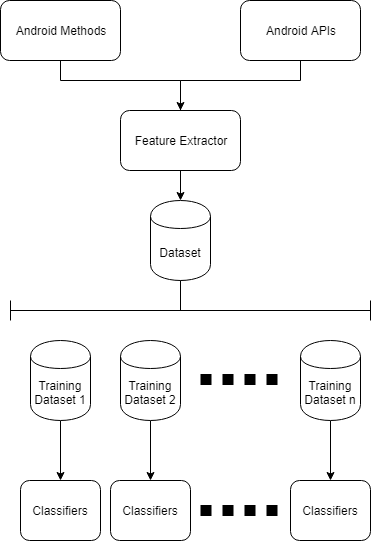
\includegraphics[width=0.5\linewidth]{images/architectures-training.png}
    \end{center}
    \caption{%
        Overview of the proposed training flow. First, the feature extractor uses Android Methods and %
        Android APIs to create a dataset, which will be sampled into other 30 different datasets that will be used %
        to train the classifiers.%
    }\label{figure:train-flow}
    \vspace{4ex}
\end{figure}

If the extraction is made using an emulator, instead of a real device, the API comes without the complete method implementation, called method stubs. As long as the taint tracker try to execute or extract runtime information from any of these methods stubs, an exception is thrown and the execution is stopped. The fully implemented methods are important due to information tracking that is done during the feature extraction, if a API method calls another method that is a source of sensitive data, the method potentially be a source of data too. Another point is that some of syntactic features are extracted from data flow inside those methods, if no method implementation were given, those features could not be computed.

In addition to the APIs, it is necessary to have a starting list of Android methods that have been hand classified, called hand annotated methods.  The feature extractor will use the hand annotated methods and the API to generate the methods features and if possible, infer the classes of non annotated methods using static taint analysis. The result of this step is the dataset used in the classification and is described in more details in Section \ref{dset_section}. With the hand annotated methods and the APIs in hand, the following step is to apply the feature extractor to each API, concatenate all the results and remove all the repeated entries, resulting in the dataset.

After the dataset creation, 30 other datasets are randomly sampled from the original, with the objective to train and evaluate the classification algorithms using a hypothesis test. Each of these datasets are subdivided into two disjoint datasets: train and test. The train dataset consists in 80\% of the original dataset and to test the model effectiveness, the test dataset have 20\% of the original samples. This is a random division done in such a way that the resultant datasets maintain the classes proportion observed in the original, if the original has 45\% of source methods, the train and test must have a proportion close to that. The datasets are created by random sample of the original one, the algorithm calculates the classes proportion and randomly selects entries to be used in train and test keeping the proportion close to the original one.

At the end of one training step, the model is evaluated with the test dataset. The whole test step is shown in Figure \ref{figure:test-flow}, for each dataset, there is a classifier to categorize the samples. This will result in a list of samples and classified labels that are going to be compared with the original label. This generates the evaluation results, consisting in precision, recall, F1 score and accuracy, the result of each metric is saved. After the the result saved, the model is overwritten and a fresh one is used to be used back in the training step. This ensures that no information is being  transferred to the next step, forgetting all the information previously learned. And at the end of 30 steps of training and test, the mean and standard deviation of each metric is calculated and reported in the results, Section \ref{result_ending}.

\begin{figure}[!h]
    \begin{center}
        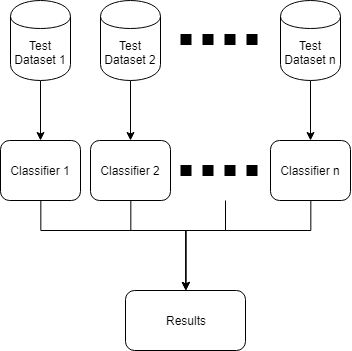
\includegraphics[width=0.5\linewidth]{images/architectures-test.png}
    \end{center}
    \caption{%
        Overview of the proposed testing flow. After the creation of datasets, the result of each classifier is used in evaluation.%
    }\label{figure:test-flow}
    \vspace{4ex}
\end{figure}

\chapter{Results}\label{chapter:results}

In this chapter, the results are exposed in the following way: Section \ref{dset_section} shows how the dataset has been created and the overall proportion of classes. Section \ref{mono} is reserved to comparison and evaluation of monolithic machine learning models, Decision Tree, K-Nearest Neighbors, Multi Layer Perceptron, Naive Bayes and Support Vector Machine. For Multiple Classifier System (MCS), the Section \ref{mcs} compares the KNORAE, KNORAU, META-DES, OLA, Single Best and Static Selection. After the comparison between Monolithic and MCS, the overall comparison is discussed in Section \ref{result_ending}.

Using the dataset described in Section \ref{dset_section} other 30 different datasets have been randomly sampled that are subdivided into two: 80\% of the original dataset for model training and 20\% to test the model effectiveness. This method intends to make a Hypothesis Test, this help to statically evaluate if a classifier is really effective when applied in this dataset. After the classifiers applied to each of the 30 datasets, the mean and standard deviation of each metric are calculated and displayed in the result tables. For each classification method, both Monolithic and MCS have its setup described in Sections \ref{mono} and \ref{mcs} to ease future replications of this work. 

Each classifier is evaluated with 4 different metrics, precision (equation \ref{precision}), recall (equation \ref{recall}), F1 score (equation \ref{f1}) and accuracy (equation \ref{accuracy}). The precision is the ratio of correctly predictions to the total predictions done. Accuracy is the ratio of correctly true predictions to the total of predictions. Recall is the ratio of correctly positive predictions to all the predictions of a class. F1 score represents the harmonic mean between precision and recall, which is a more meaningful metric than the mean between precision and recall \cite{sasaki2007truth}. True positives are all instances of a class $C$ that are correctly classified. True negatives are all instances that do not belong to $C$ and are correctly classified. False positives of a class $C$ are the instances of other classes that has been classified as $C$. False negatives are instances of $C$ that has been classified as not belonging to $C$.

\begin{multicols}{2}%
    \noindent%
    {%
    \begin{equation} \label{precision} precision = \frac{TP}{TP+FP} \end{equation}%
    \begin{equation} \label{recall} recall = \frac{TP}{TP+FN} \end{equation}%
    }%
    {%
    \begin{equation} \label{f1} F1 = \frac{2 \times recall \times precision}{recall + precision} \end{equation}%
    \begin{equation} \label{accuracy} accuracy = \frac{TP+TN}{TP+TN+FP+FN} \end{equation}%
    }%
\end{multicols}

\section{Dataset}\label{dset_section}

The dataset created in this work uses the feature extractor developed by \cite{rasthofer2014machine}. The extractor creates meaningful information using the Android methods names and their real implementation in the Android API. As result, the extractor gives the method class, if has been hand annotated, and a list of features. These features are lexical, semantic and syntactic, which contains information about the method name, parameters, return type, method modifiers, classes modifiers, if exists data flow in the method return or parameters and the required permissions.

Lexical features follows the idea that the Android APIs adopts a specific coding style, described in \cite{androidcoderef}. Extracting if a method name or parameter name contains certain strings can lead to the prediction of the method class. For syntactic features, the feature extractor evaluates if exists data flow inside a method using Taint Analysis, discussed in Chapter \ref{chapter:background}. Finally, the semantic features are information extracted from classes modifiers, such as private, public, protected and types of variables, arguments and methods returns.

As result, the feature extractor gives 215 features, consisting in 53 semantic, 45 syntactic and 117 lexical features, extracted from the Android API Level 3 to Level 27, excluding APIs Level 18 and 20 which complete binaries could not be found. The features extracted consists in boolean variables represented in 12 categories, the dataset also contains the full method name and signature but is not being used in classification. The lexical features are extracted by analyzing the stream of characters from the source code, syntactic features represents the dependency of data and control for code variables and methods, semantic features consists in the types and modifiers for variables, methods and classes \cite{aho2003compilers}.

\begin{table}[hb!]
    \centering
    \renewcommand{\arraystretch}{1.8}
    \begin{tabular}{p{2.5cm}p{2.5cm}p{2.5cm}p{2cm} }
        \toprule
        Source & Sink & Neithernor & Total\\
        \midrule
        375 (55.97) & 176 (26.27) & 119 (17.76) & 670 (100)\\ [1ex]
        \bottomrule
        \end{tabular}
        \caption{%
        The final dataset proportion without duplicated entries.%
        }\label{dset_prop}
\end{table}

With that said, Table \ref{dset_prop} shows the proportion of each class for the dataset. First we evaluate the feature extractor using the Android API 17, same API used in \cite{rasthofer2014machine} and we could extract a total of 535 methods, consisting in 131 sinks, 88 sources and 316 neither nor. Using Android API Level 3 to Level 27, excluding APIs Level 18 and 20, we extracted 670 methods in total when dropping repeated entries (Dropped Entries dataset), being 176 sinks, 119 sources and 375 neither nor. It is important to observe that none of the dataset entries are duplicated, but if we look closely to the dataset, the same method can have different value of features through different APIs, as shown in Figure \ref{menthod_though_apis}. So, considering method names as duplication factor (Dropped Names dataset), we end up with only 543 method, unlike the 670 for the Dropped Entries, disperse in 134 sinks, 87 sources and 322 neithernor. As different feature values consists in different entries, despite the same method name, we considered the larger dataset in order to have a bigger quantity of data to be analyzed, so we only dropped entries that are really duplicated. Sometimes the feature extractor could not infer syntactic features for a method, these entries are also removed from the dataset to keep the dataset integrity.

Due to the repetition of methods in different APIs, and not necessarily the same features repeated, drop entries with repeated method names reduces the quantity of methods available to be trained. So we chose as default dataset for the evaluation the dataset with dropped repeated entries, this dataset have more information to be learned and already guarantee the division in training and testing to be disjoint as have no repetition.

\begin{figure}[h!]
    \centering
    \renewcommand{\arraystretch}{1.8}
    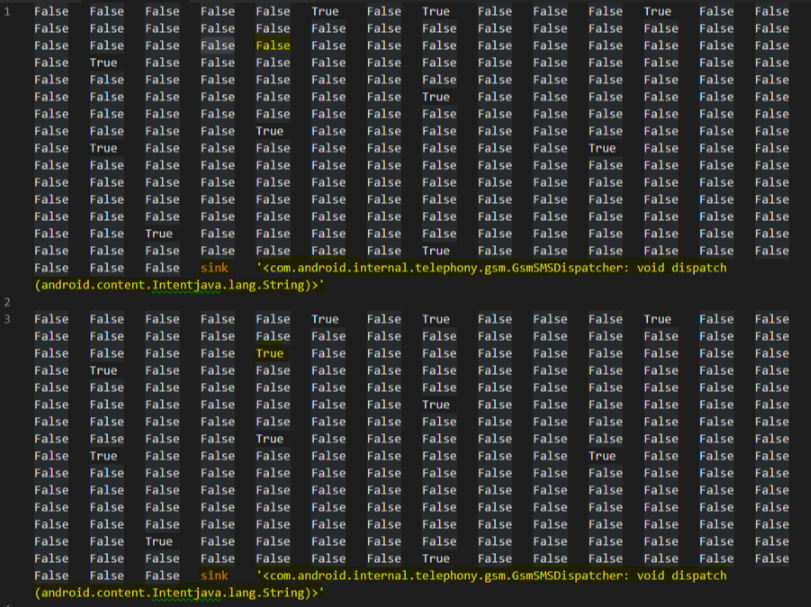
\includegraphics[width=0.9\linewidth]{images/menthod_though_apis.png}
    \caption{%
    Methods through different API Levels. We can observe in yellow the feature "Method modifier is PUBLIC" and the full method name. Even for different features values, marked in green, the method still belongs to the sink class.%
    }
\end{figure}\label{menthod_though_apis}

\section{Monolithic}\label{mono}

For the Monolithic classifiers, we have the Decision Tree, Multinomial and Bernoulli Naive Bayes, K-Nearest Neighbor (KNN), Support Vector Machine (SVM), Multi-Layer Perceptron and Random Forest.

The setup for Decision Tree is the split strategy to select the most relevant feature with Gini Impurity as criterion. In Multinomial and Bernoulli Naive Bayes we choose a $\alpha$ of 1. For KNN, we use 5 as the number of neighbors and a uniform weight for the neighbor points. The SVM has L2 as penalty, linear kernel, $C = 1$ and tolerance of $10^{-4}$. For MLP we used L2 regularization with alpha of $10^{-4}$, 1000 neurons in hidden layer, no early stopping, activation layer as relu, max of 1000 iterations and tolerance of $10^{-4}$. For Random Forests we are using 10 estimators, the minimum samples to split is 2 and Gini Impurity as criterion. The parameters can also be seen in Table \ref{table:monolithic_params}.

\begin{table}[h!]
    \centering
    \renewcommand{\arraystretch}{1.8}
    \begin{tabular}{ p{4cm}p{1.62cm}|p{1.5cm}|p{1.5cm}|p{1.5cm}|p{1.5cm} }
        \toprule
        Model & \multicolumn{5}{c}{Parameters} \\
        \midrule
        Decision Tree & criterion Gini & spliter best & & &\\
        Multinomial NB & $\alpha = 1$ & & & &\\
        Bernoulli NB & $\alpha = 1$ & & & &\\
        KNN & $ k = 5 $ & uniform weight & & &\\
        Linear SVM & penalty L2 & $C = 1$ & tolerance $10^{-4}$ & &\\
        MLP  & $ \alpha = 10^{-4} $ & reg. L2  & activation relu & tolerance $10^{-4}$ & hidden neurons 1000 \\
        Random Forest & criterion Gini & samples 2 & estimators 10 & & \\ [1ex]
        \bottomrule
        \end{tabular}
        \caption{%
        Parameters for Monolithic Classifiers%
        }\label{table:monolithic_params}
\end{table}

\begin{table}[h!]
    \centering
    \renewcommand{\arraystretch}{1.8}
    \begin{tabular}{ p{3cm}p{2.8cm}p{2.8cm}p{2.8cm}p{2.8cm} }
        \toprule
        Model & Precision & Recall & F1 Score & Accuracy \\
        \midrule
        Decision Tree & 0.8474 (0.0505) & 0.8388 (0.0549) & 0.8410 (0.0357) & 0.8497 (0.0217) \\
        Multinomial NB & 0.8297 (0.0595) & 0.8211 (0.0552) & 0.8231 (0.0416) & 0.8387 (0.0282) \\
        Bernoulli NB & 0.8307 (0.0609) & 0.8180 (0.0561) & 0.8220 (0.0424) & 0.8378 (0.0271) \\
        KNN & 0.8635 (0.0547) & 0.7991 (0.0657) & 0.8217 (0.0484) & 0.8432 (0.0307) \\
        Linear SVM & 0.8920 (0.0559) & 0.8718 (0.0539) & 0.8796 (0.0436) & 0.8859 (0.0284) \\
        MLP & 0.8936 (0.0547) & \textbf{0.8759 (0.0541)} & \textbf{0.8830 (0.0437)} & \textbf{0.8908 (0.0302)} \\
        Random Forest & \textbf{0.8953 (0.0568)} & 0.8522 (0.0605) & 0.8684 (0.0438) & 0.8791 (0.0309) \\ [1ex]
        \bottomrule
        \end{tabular}
        \caption{%
        Result for Monolithic Classifiers, Mean (Standard Deviation), the best classifier for each metric is highlighted in bold. Using the %
        }\label{table:result_monolithic}
\end{table}

The Table \ref{table:result_monolithic} is showing the results for Monolithic Classifiers. We can observe that the MLP has better results overall, just behind of Random Forest in precision by 0,0017. This interval is within the confidence interval, the standard deviation of MLP and Random Forest have the same approximation of 0.05. We can also observe that the SMV is close to MLP and Random Forest in all metrics, this is an evidence that SVM can solve this problem as well as these two.
\section{Multiple Classifier System}\label{mcs}

For the Multiple Classifier System we used KNORAE, KNORAU, META-DES, OLA, Single Best and Static Selection. Each of these algorithms has the objective to select the best classifier in a set, in our evaluation, we are using a pool of 100 classifiers of the same base class.

The base classifier classes used are Perceptron and Decision Tree, in all ensemble algorithms we use the same base classifier configuration. For Perceptron we used no regularization, no early stopping, max of 1000 iterations and tolerance of $10^{-1}$. For Decision Tree, the split strategy is to select the most relevant feature with Gini Impurity as criterion. For ensemble algorithms, the KNORAE and KNORAU parameters were KNN to estimate the classifier competence using 7 neighbors, with no dynamic pruning and no indecision region. For META-DES, we are using Multinomial Naive Bayes as meta-classifier, 5 output profiles to estimate the competence using a KNN with 7 neighbors to decide the region of competence. And finally, static selection, we are choosing 50\% of the base classifiers. All parameters can be seen in Table \ref{table:mcs_params}.

\begin{table}[h!]
    \centering
    \renewcommand{\arraystretch}{1.8}
    \begin{tabular}{ p{5cm}p{3cm}|p{3cm}|p{3cm} }
        \toprule
        Model & \multicolumn{3}{c}{Parameters} \\
        \midrule
        Perceptron & max iterations \newline 1000 & tolerance $10^{-4}$ & \\
        Decision Tree & criterion Gini & spliter best & \\
        \midrule
        KNORAE and KNORAU & $k = 7$ & no prune & no indecision \\
        META-DES & Multinom. NB & $K_p = 5$ & $k = 7$ \\
        Static Selection & selection 50\% & & \\
        \bottomrule
        \end{tabular}
        \caption{%
        Parameters for Multiple Classifier System%
        }\label{table:mcs_params}
\end{table}

In Table \ref{mcs_dt_table} is presented the MCS algorithms using Decision Tree classifier. We can observe a better mean result using META-DES in all metrics. Considering the mean and standard deviation, the results for KNORAE, OLA, Static Selection and META-DES are very close to the same interval.

When using Perceptron as main classifier, Table \ref{mcs_perceptron_table}, we can observe that KNORAE and META-DES have the best mean results, META-DES has better Precision ad Accuracy and KNORAE has better Recall and F1 Score. But also, when considering the mean and standard deviation, the results are in the same range comparing KNORAE, KNORAU, OLA and Static Selection.Comparing both Decision Tree and Perceptron results in MCS, the results are very close, having 0.8665(0.0316) as F1 Score for the best Perceptron MCS (KNORAE) and 0.8741(0.0284) for the best Decision Tree MCS (META-DES), a difference of just 0.0086.

\begin{table}[h!]
    \centering
    \renewcommand{\arraystretch}{1.8}
    \begin{tabular}{ p{3cm}p{2.8cm}p{2.8cm}p{2.8cm}p{2.8cm} }
        \toprule
        Model & Precision & Recall & F1 Score & Accuracy \\
        \midrule
        KNORAE &            0.8602 (0.0517) & 0.8395 (0.0656) & 0.8469 (0.0455) & \textbf{0.8580 (0.0306)} \\
        KNORAU &            0.8377 (0.0557) & 0.8071 (0.0743) & 0.8181 (0.0495) & 0.8313 (0.0321) \\
        META-DES &          \textbf{0.8609 (0.0551)} & \textbf{0.8423 (0.0639)} & \textbf{0.8492 (0.0482)} & 0.8575 (0.0344) \\
        OLA &               0.8263 (0.0589) & 0.8104 (0.0667) & 0.8158 (0.0532) & 0.8306 (0.0387) \\
        Single Best &       0.7609 (0.0739) & 0.7356 (0.0994) & 0.7423 (0.0688) & 0.7629 (0.0447) \\
        Static Selection &  0.8424 (0.0579) & 0.8099 (0.0741) & 0.8213 (0.0492) & 0.8338 (0.0341) \\ [1ex]
        \bottomrule
        \end{tabular}
        \caption{%
        Result for Multiple Classifier System, Mean (Standard Deviation), using Decision Tree as main classifier with most relevant feature as split strategy and Gini Impurity as criterion. The best classifier for each metric is highlighted in bold%
        }\label{mcs_dt_table}
\end{table}

\begin{table}[h!]
    \centering
    \renewcommand{\arraystretch}{1.8}
    \begin{tabular}{ p{3cm}p{2.8cm}p{2.8cm}p{2.8cm}p{2.8cm} }
        \toprule
        Model & Precision & Recall & F1 Score & Accuracy \\
        \midrule
        KNORAE &            0.8607 (0.0556) & \textbf{0.8368 (0.0678)} & \textbf{0.8452 (0.0471)} & \textbf{0.8570 (0.0273)} \\
        KNORAU &            0.8446 (0.0562) & 0.8148 (0.0581) & 0.8260 (0.0451) & 0.8386 (0.0301) \\
        META-DES &          \textbf{0.8748 (0.0559)} & 0.8167 (0.0700) & 0.8375 (0.0518) & 0.8525 (0.0335) \\
        OLA &               0.8418 (0.0580) & 0.8216 (0.0550) & 0.8282 (0.0413) & 0.8410 (0.0268) \\
        Single Best &       0.7913 (0.0753) & 0.7552 (0.1007) & 0.7644 (0.0688) & 0.7866 (0.0451) \\
        Static Selection &  0.8523 (0.0593) & 0.8158 (0.0717) & 0.8291 (0.0512) & 0.8438 (0.0329) \\ [1ex]
        \bottomrule
        \end{tabular}
        \caption{%
        Result for Multiple Classifier System, Mean (Standard Deviation), using Perceptron as main classifier using no regularization, no early stopping, max of 1000 iterations and tolerance of $10^{-1}$. The best classifier for each metric is highlighted in bold%
        }\label{mcs_perceptron_table}
\end{table}
\section{Final Considerations}\label{result_ending}

With the Monolithic and MCS compared, now we must compare the best Monolithic and the best MCS to fully understand which model is the most indicated to solve the problem of Android API methods categorization. Table \ref{table:overall_comp} show the performance of each classifier: MLP and METADES using Decision Tree, and we can see that the MLP has better results in all the metrics.

\begin{table}[hb]
    \centering
    \renewcommand{\arraystretch}{1.8}
    \begin{tabular}{ p{3cm}p{2.8cm}p{2.8cm}p{2.8cm}p{2.8cm} }
        \toprule
        Model & Precision & Recall & Accuracy & F1 Score \\
        \midrule
        MLP &       \textbf{0.8838 (0.0474)} & \textbf{0.8709 (0.0544)} & \textbf{0.8758 (0.0426)} & \textbf{0.8856 (0.0287)} \\
        META-DES \newline Decision Tree &  0.8609 (0.0551) & 0.8423 (0.0639) & 0.8492 (0.0482) & 0.8575 (0.0344) \\
        \bottomrule
    \end{tabular}
    \caption{%
        The best of Monolithic compared to the best of MCS, Mean (Standard Deviation). The best classifier for each metric is highlighted in bold.
        %
    }\label{table:overall_comp}
\end{table}

\begin{table}[!ht]
    \centering
    \renewcommand{\arraystretch}{1.8}
    \begin{tabular}{ p{2.2cm}p{0.8cm}p{2.7cm}p{2.7cm}p{2.7cm}p{2.7cm} }
        \toprule
        Model & Class & Precision & Recall & Accuracy & F1 Score \\
        \midrule
        \multirow{3}{*}{MLP}
        & (1) & 0.8792 (0.0597) & \textbf{0.8708 (0.0786)} & \textbf{0.8731 (0.0577)} & \textbf{0.8856 (0.0287)} \\
        & (2) & \textbf{0.8803 (0.0486)} & \textbf{0.8219 (0.0598)} & \textbf{0.8489 (0.0450)} & \textbf{0.8856 (0.0287)} \\
        & (3) & \textbf{0.8920 (0.0339)} & \textbf{0.9200 (0.0248)} & \textbf{0.9055 (0.0251)} & \textbf{0.8856 (0.0287)} \\
        \midrule
        \multirow{3}{*}{\shortstack{METADES\\Decision Tree }}
        & (1) & \textbf{0.8870 (0.0658)} & 0.8611 (0.0889) & 0.8702 (0.0580) & 0.8575 (0.0344) \\
        & (2) & 0.8344 (0.0636) & 0.7676 (0.0691) & 0.7983 (0.0579) & 0.8575 (0.0344) \\
        & (3) & 0.8614 (0.0361) & 0.8982 (0.0338) & 0.8790 (0.0288) & 0.8575 (0.0344) \\
        \bottomrule
        \end{tabular}
        \caption{%
        C The best of Monolithic compared to the best of MCS, Mean (Standard Deviation). The Class (1) represents the Source methods, Class (2) are the Sink methods and (3) Neithernor. The best classifier for each metric and class is highlighted in bold.
        %
        }\label{table:per_class_overall_comp}
\end{table}

Looking deep to the results for each class, we can observe in Table \ref{table:per_class_overall_comp} that the MLP has a better score in the majority of classes and metrics and METADES using Decision Tree as base classifier has better Precision when classifying the Source methods. If we look at the standard deviation, we can conclude that the classifiers are also in the same interval for all the metrics, this is another evidence that a simpler algorithm can address this problem.

\chapter{Conclusion}


% Uncomment to proposal
% \chapter{Introduction}
Every program computes on either sensitive data or non-sensitive data. Sensitive is any data that can be used to 
identify the user or any private user information, such as photos, International Mobile Equipment Identity (IMEI) 
nd biometric data. Non-sensitive data is any dynamic information that do not identify the user, oftenly this kind 
of information if public or shared, such as application source code.

In an application, data follows a specific flow, first it is acquired from data sources and sent to data 
sinks \citep{mccabe2003network}. Data sources, in the context of mobile and IoT devices, are defined as method 
calls that read data from shared resources such as phone calls, screenshots, sensor polling data from ambient, 
device identification numbers \citep{rasthofer2014machine}. Data sinks are methods calls that have at least one 
argument, this argument is non-constant data from the source code \citep{rasthofer2014machine}. The data sink can be
an interface to the user or system API for communication to other devices or store data \citep{viet2010specifying}.

Dynamic Flow Enforcement are techniques that tracks and enforces information flow during the application runtime. 
These methods relies on Taint Analysis to track possible sensitive data flow to untrusted sinks. Taint Analysis 
marks every sensitive data gathered from a source and every other variable that inherit any operation 
from the tainted data, in the end, if any tainted variable is accessed by a sink method, the information has 
leaked and the analysis gives a detailed path through which the data passed. During the tracking, there are 
different methods to enforce in runtime that the data will not leak, \cite{fernandes2016flowfence} uses 
virtualization to guarantee that the data will only operate in the controlled environment and \cite{sun2017data} 
declassifying information before it is computed in trusted methods or if reach a trusted API.

Static Flow Enforcement starts by creating abstract models of the application code to provide a simpler 
representation \citep{myers1999jflow}, using frameworks like Soot \citep{vallee2000optimizing}. Then, this model 
will be used in control-flow, data-flow and points-to analysis to observe the application control, data sequence 
and compute static abstractions for variables \cite{li2017static}. These methods are implemented and used in 
DroidSafe \cite{gordon2015information}. JFlow \cite{myers1999jflow} inserts statically checked and secured code 
when the application computes on sensitive data.

Both Static and Dynamic Flow Enforcement techniques require information of which methods is a source of sensitive 
data and which is a data sink. This is used to identify if a sink method is truly leaking sensitive data or not. So,
lists containing sources and sinks of sensitive data are hand created, but this solution is impractical considering 
a huge API like the Android API \cite{rasthofer2014machine}.

Considering that issue, Rasthofer et al. \cite{rasthofer2014machine} proposed to use machine learning to 
automatically create a categorized list of sources and sinks methods to be used in Flow Enforcement techniques.
The list consists in methods classified into Flow Classes and Android Method Categories. The Flow Classes are 
source of sensitive data, or just source, and sink of data, but also, the method can be neither source or sink. For 
Android Methods Categories, there are 12 different classes: account, Bluetooth, browser, calendar, contact, 
database, file, network, NFC, settings, sync, a unique identifier, and no category if the method does not belong to 
any of the previous.

The authors shortly compared Decision Trees and Naive Bayes with the SVM and choosed to use SVM to create the 
categorized list of sources and sinks, as SVM showed to be more precise in categorize the Android methods. 

To classify, the authors utilize features extracted from the methods, like the method name, if the method has 
parameters, the return value type, parameter type, if the parameter is an interface, method modifiers, class 
modifiers, class name, if the method returns a value from another source method, if one parameter flows into a sink 
method, if a method parameters flows into a abstract sink and the method required permission. 

To categorize the methods, were used features like class name, method invocation, body contents, parameter type and 
return value type. After that, the methods list is generated containing if it is a sink, source and the method 
category.

% \chapter{Objectives}
This work has two main objectives: generate a public database containing methods from Android APIs and evaluate the 
performance of the most used classification algorithms on this database. The methods should be classified into any 
of the two Flow Classes, source or sink, or neither.

The motivation behind the database creation comes when \cite{rasthofer2014machine} developed the initial 
classification work. Their objective were create a machine-learning solution to identify sources and sink methods 
from the code of any Android API. So, every time that you wanted to test other classification algorithms, you had 
to extract the methods and features at every execution. Then, create a public database extract knowledge and 
develop better solutions to this problem is very likely.

The objective of evaluate different classification algorithms comes as \cite{rasthofer2014machine} shows results 
for only three classification algorithms, SVM, Decision Tree and Naive Bayes. From that, emerged the question if 
other classification algorithms have better results in this database. So, the second objective is to evaluate the 
most used classifiers in the literature, SVM, Naive Bayes, Decision Trees, MLP, KNN, including ensemble 
classifications methods.

% \chapter{Methodology}
As first objective, the dataset will be created using the feature extractor developed by 
\cite{rasthofer2014machine}. The extractor creates meaningful information using the Android methods names and 
their real implementation in the Android API. As result, the extractor gives the method class, if has been hand 
annotaded, and a list of features. These features are semantic and syntactic features, containing information about 
the method name, parameters, return type, method and classes modifiers, class modifiers, if exists data flow in the 
method return or parameters and the required permissions.

The extractor will be used in many Android APIs as possible, since there are a low quantity of hand annotated 
methods, it is important to extract as many methods from classes as possible. It is possible to have duplicated 
methods at the end of this evaluation due to backward compatibility, so, methods from older APIs will be 
overwritten.

The methods used in the comparison will be SVM, Naive Bayes, Decision Trees, MLP, KNN, and ensemble classifications 
methods, which will be evaluated in 30 datasets sampled from the original. Each of these datasets are 
subdivided into train dataset and test dataset, containing 80\% of the original dataset for model training and 20\% 
for test the model effectiveness. They must maintain the classes proportion observed in the original dataset, if 
the original has 45\% of source methods, the train and test must have a proportion close to that. Create these 
datasets are important to make a Hypothesis Test, this help to statically evaluate if a classifier is really 
effective when applied in this dataset. The proposed evaluation flow is shown in figure \ref{flow}.

\begin{multicols}{2}%
    \noindent%
    {%
    \begin{equation} \label{precision} precision = \frac{TP}{TP+FP} \end{equation}%
    \begin{equation} \label{accuracy} accuracy = \frac{TP+TN}{TP+TN+FP+FN} \end{equation}%
    }%
    {%
    \begin{equation} \label{recall} recall = \frac{TP}{TP+FN} \end{equation}%
    \begin{equation} \label{f1} F1 = \frac{2 \times recall \times precision}{recall + precision} \end{equation}%
    }%
\end{multicols}

Each classifier will be evaluated using precision, accuracy, recall and F1 score. The precision, equation 
\ref{precision}, is the ratio of correctly predictions to the total predictions done. Accuracy, equation 
\ref{accuracy}, is the ratio of correctly true predictions to the total of true predictions. Recall, equation 
\ref{recall} is the ratio of correctly positive predictions to all the predictions of a class. F1, equation 
\ref{f1}, score represents the harmonic mean between precision and recall \cite{sasaki2007truth}.

We can rewrite precision, accuracy, recall and F1 score in the equations above, using true positives (TP), true 
negatives (TN), false positives (FP) and false negatives (FN). True positives are all instances of a class $C$ that 
are correctly classified. True negatives are all instances that do not belong to $C$ and are correctly classified. 
False positives of a class $C$ are the instances of other classes that has been classified as $C$. False negatives 
are instances of $C$ that has been classified as not belonging to $C$.

\begin{figure}[!h]
    \begin{center}
        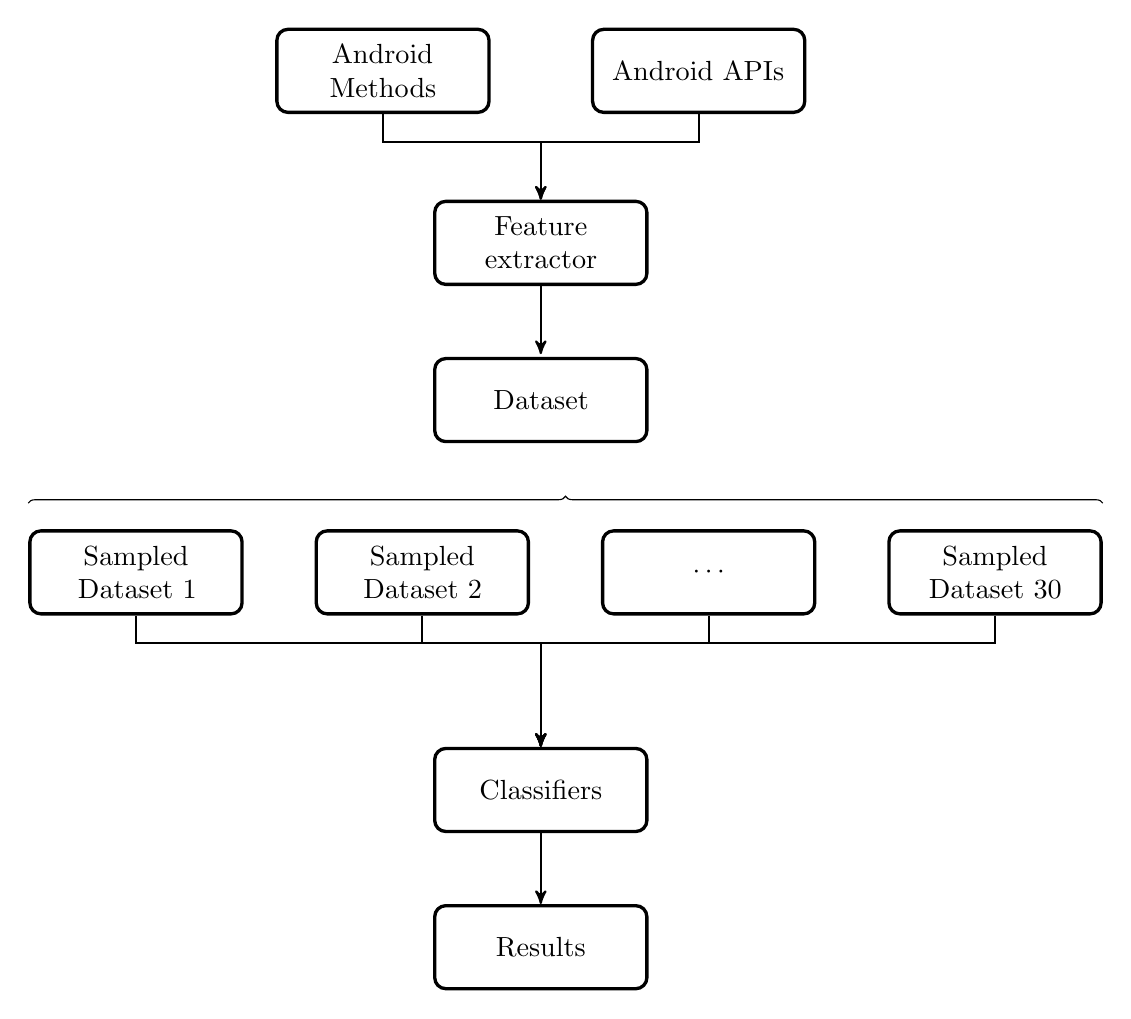
\begin{tikzpicture} [node distance=.9cm, start chain=going below]
    \node[punktchain] (ext) {Feature extractor};
    \node[punktchain, join] (dset) {Dataset};
    \node[punktchain, below left = of dset] (sdset2) at (0.5, -3) {Sampled Dataset 2};

    %We need to redefine the join-style to have the -> turn out right
    \begin{scope}[start branch=venstre, every join/.style={->, thick, shorten <=1pt}]
        \node[punktchain, on chain=going left] (sdset1) {Sampled Dataset 1};
    \end{scope}

    \node[punktchain, right = of sdset2] (dots) {$\cdots$};

    \begin{scope}[start branch=hoejre]
        \node[punktchain, on chain=going right] (sdset30) {Sampled Dataset 30};
    \end{scope}
    
    \node[punktchain, below = of dset] (class) at (0, -5.5) {Classifiers};
    % Now that we have finished the main figure let us add some "after-drawings"
    %% First, let us connect (finans) with (disk). We want it to have
    %% square corners.
    \draw[|-,-|,->, thick,] (sdset1.south) |-+(0,-1em)-| (class.north);
    \draw[|-,-|,->, thick,] (sdset30.south) |-+(0,-1em)-| (class.north);
    \draw[|-,-|,->, thick,] (dots.south) |-+(0,-1em)-| (class.north);
    \draw[|-,-|,->, thick,] (sdset2.south) |-+(0,-1em)-| (class.north);
    % Now, let us add some braches. 
    %% No. 1
    \draw[tuborg] let \p1=(sdset1.west), \p2=(sdset30.east) in ($(\x1,\y1+2.5em)$) -- ($(\x2,\y2+2.5em)$);

    \begin{scope}
        \node[punktchain, above left = of ext] (meth) at (0, 1) {Android Methods};
        \node[punktchain, above right = of ext] (api) at (0, 1) {Android APIs};

        \draw[|-,-|,->, thick,] (meth.south) |-+(0,-1em)-| (ext.north);
        \draw[|-,-|,->, thick,] (api.south) |-+(0,-1em)-| (ext.north);
    \end{scope}

    \node[punktchain, below = of class] (res) {Results};
    \draw[|-,-|,->, thick,] (class.south) |-+(0,-1em)-| (res.north);
\end{tikzpicture}
    \end{center}
    \caption{%
        Overview of the proposed evaluation flow. First, the feature extractor uses Android Methods and %
        Android APIs to create a dataset, which will be sampled into other 30 different datasets that will be used %
        to evaluate the Classifiers.%
    }\label{flow}
\end{figure}


% \chapter{Schedule}

\begin{center}
    \begin{table}[htp]
        \begin{tabular}{l|c|c|c|c|c|c|c|c|c|c|c|c|c|c|c|c|}
        \cline{2-17}
        & \multicolumn{16}{c|}{\cellcolor[HTML]{C0C0C0}{\color[HTML]{333333} Period}} \\ \hline
        \multicolumn{1}{|l|}{\cellcolor[HTML]{C0C0C0}Activity} & \multicolumn{2}{c|}{August} & \multicolumn{4}{c|}{September} & \multicolumn{4}{c|}{October} & \multicolumn{4}{c|}{November} & \multicolumn{2}{c|}{December} \\ \hline
        \multicolumn{1}{|l|}{Literature Review}                & x            & x            & x      &       &       &       &       &       &       &      &       &       &       &       &               &               \\ \hline
        \multicolumn{1}{|l|}{Dataset creation}                 &              &              & x      & x     & x     & x     &       &       &       &      &       &       &       &       &               &               \\ \hline
        \multicolumn{1}{|l|}{Algorithm studies}                &              &              &        &       &       & x     & x     & x     &       &      &       &       &       &       &               &               \\ \hline
        \multicolumn{1}{|l|}{Experiments}                      &              &              &        &       &       &       & x     & x     & x     & x    &       &       &       &       &               &               \\ \hline
        \multicolumn{1}{|l|}{Evaluation}                       &              &              &        &       &       &       &       &       & x     & x    & x     &       &       &       &               &               \\ \hline
        \multicolumn{1}{|l|}{Writing}                          &              &              &        &       &       &       &       &       &       & x    & x     & x     & x     & x     & x             &               \\ \hline
        \multicolumn{1}{|l|}{Presentation preparation}         &              &              &        &       &       &       &       &       &       &      &       &       &       &       & x             & x             \\ \hline
        \end{tabular}
    \end{table}
\end{center}


% \chapter{Possível Avaliador}

Paulo Salgado Gomes de Mattos Neto

\begin{references}
  \bibliography{references}
\end{references}

% References


% Appendix

\theappendix
'<Base name of class package name: accounts>'	'<Base name of class package name: io>'	'<Base name of class package name: music>'	'<Base name of class package name: telephony>'	'<Base name of class package name: webkit>'	'<Method has parameters>'	'<Method is lone getter or setter>'	'<Method is part of a ABSTRACT class>'	'<Method is part of a FINAL class>'	'<Method is part of a PRIVATE class>'	'<Method is part of a PROTECTED class>'	'<Method is part of a PUBLIC class>'	'<Method is part of a STATIC class>'	'<Method is part of an anonymous class>'	'<Method is part of class android.app.Activity>'	'<Method is part of class android.app.BroadcastReceiver>'	'<Method is part of class android.app.ContentProvider>'	'<Method is part of class android.app.Service>'	'<Method is part of class android.content.ContentResolver>'	'<Method is part of class android.content.Context>'	'<Method is part of class that contains the name com.google.common.io>'	'<Method is part of class that contains the name java.io.>'	'<Method is part of class that ends with Context>'	'<Method is part of class that ends with Factory>'	'<Method is part of class that ends with Handler>'	'<Method is part of class that ends with Loader>'	'<Method is part of class that ends with Manager>'	'<Method is part of class that ends with Service>'	'<Method is part of class that ends with View>'	'<Method is thread runner>'	'<Method modifier is FINAL>'	'<Method modifier is PROTECTED>'	'<Method modifier is PUBLIC>'	'<Method modifier is STATIC>'	'<Method name ends with Messenger>'	'<Method name starts with <init>>'	'<Method name starts with add>'	'<Method name starts with apply>'	'<Method name starts with bind>'	'<Method name starts with clear>'	'<Method name starts with close>'	'<Method name starts with delete>'	'<Method name starts with disable>'	'<Method name starts with dispatch>'	'<Method name starts with do>'	'<Method name starts with dump>'	'<Method name starts with enable>'	'<Method name starts with finish>'	'<Method name starts with get>'	'<Method name starts with handle>'	'<Method name starts with insert>'	'<Method name starts with is>'	'<Method name starts with load>'	'<Method name starts with note>'	'<Method name starts with notify>'	'<Method name starts with onClick>'	'<Method name starts with open>'	'<Method name starts with perform>'	'<Method name starts with process>'	'<Method name starts with put>'	'<Method name starts with query>'	'<Method name starts with register>'	'<Method name starts with release>'	'<Method name starts with remove>'	'<Method name starts with request>'	'<Method name starts with restore>'	'<Method name starts with run>'	'<Method name starts with send>'	'<Method name starts with set>'	'<Method name starts with start>'	'<Method name starts with supply>'	'<Method name starts with toggle>'	'<Method name starts with unregister>'	'<Method name starts with update>'	'<Method returns constant>'	'<Method starts with on and has void/bool return type>'	'<Parameter is interface>'	'<Parameter to abstract sink>'	'<Parameter to sink method adjust>'	'<Parameter to sink method bind>'	'<Parameter to sink method broadcast>'	'<Parameter to sink method clear>'	'<Parameter to sink method com.android.internal.telephony.CommandsInterface>'	'<Parameter to sink method connect>'	'<Parameter to sink method create>'	'<Parameter to sink method delete>'	'<Parameter to sink method dial>'	'<Parameter to sink method disable>'	'<Parameter to sink method dispatch>'	'<Parameter to sink method dump>'	'<Parameter to sink method enable>'	'<Parameter to sink method enqueue>'	'<Parameter to sink method insert>'	'<Parameter to sink method notify>'	'<Parameter to sink method onCreate>'	'<Parameter to sink method perform>'	'<Parameter to sink method println>'	'<Parameter to sink method put>'	'<Parameter to sink method remove>'	'<Parameter to sink method replace>'	'<Parameter to sink method restore>'	'<Parameter to sink method save>'	'<Parameter to sink method send>'	'<Parameter to sink method set>'	'<Parameter to sink method setup>'	'<Parameter to sink method show>'	'<Parameter to sink method start>'	'<Parameter to sink method sync>'	'<Parameter to sink method transact>'	'<Parameter to sink method update>'	'<Parameter to sink method write>'	'<Parameter type contains android.content.contentresolver>'	'<Parameter type contains android.content.context>'	'<Parameter type contains android.content.intent>'	'<Parameter type contains android.database.cursor>'	'<Parameter type contains android.filterfw.core.filtercontext>'	'<Parameter type contains android.net.uri>'	'<Parameter type contains com.android.inputmethod.keyboard.key>'	'<Parameter type contains com.google.common.io>'	'<Parameter type contains event>'	'<Parameter type contains java.io.>'	'<Parameter type contains java.io.filedescriptor>'	'<Parameter type contains java.lang.string>'	'<Parameter type contains observer>'	'<Parameter type contains writer>'	'<Permission name is ACCESS_COARSE_LOCATION>'	'<Permission name is ACCESS_FINE_LOCATION>'	'<Permission name is ACCESS_LOCATION_EXTRA_COMMANDS>'	'<Permission name is ACCESS_NETWORK_STATE>'	'<Permission name is ACCESS_WIFI_STATE>'	'<Permission name is ADD_VOICEMAIL>'	'<Permission name is AUTHENTICATE_ACCOUNTS>'	'<Permission name is BACKUP>'	'<Permission name is BLUETOOTH>'	'<Permission name is BLUETOOTH_ADMIN>'	'<Permission name is BROADCAST_STICKY>'	'<Permission name is CALL_PHONE>'	'<Permission name is CALL_PRIVILEGED>'	'<Permission name is CAMERA>'	'<Permission name is CHANGE_CONFIGURATION>'	'<Permission name is CHANGE_NETWORK_STATE>'	'<Permission name is CHANGE_WIFI_STATE>'	'<Permission name is CLEAR_APP_USER_DATA>'	'<Permission name is DEVICE_POWER>'	'<Permission name is DISABLE_KEYGUARD>'	'<Permission name is DUMP>'	'<Permission name is GET_ACCOUNTS>'	'<Permission name is GET_TASKS>'	'<Permission name is GLOBAL_SEARCH>'	'<Permission name is INTERNET>'	'<Permission name is KILL_BACKGROUND_PROCESSES>'	'<Permission name is MANAGE_ACCOUNTS>'	'<Permission name is MANAGE_APP_TOKENS>'	'<Permission name is MODIFY_AUDIO_SETTINGS>'	'<Permission name is MODIFY_PHONE_STATE>'	'<Permission name is MOUNT_UNMOUNT_FILESYSTEMS>'	'<Permission name is NFC>'	'<Permission name is READ_CALENDAR>'	'<Permission name is READ_CALL_LOG>'	'<Permission name is READ_CONTACTS>'	'<Permission name is READ_EXTERNAL_STORAGE>'	'<Permission name is READ_HISTORY_BOOKMARKS>'	'<Permission name is READ_PHONE_STATE>'	'<Permission name is READ_SMS>'	'<Permission name is READ_SOCIAL_STREAM>'	'<Permission name is READ_SYNC_SETTINGS>'	'<Permission name is READ_SYNC_STATS>'	'<Permission name is READ_USER_DICTIONARY>'	'<Permission name is REBOOT>'	'<Permission name is RECEIVE_BOOT_COMPLETED>'	'<Permission name is RECEIVE_SMS>'	'<Permission name is RECORD_AUDIO>'	'<Permission name is RESTART_PACKAGES>'	'<Permission name is SEND_SMS>'	'<Permission name is SET_DEBUG_APP>'	'<Permission name is SET_TIME_ZONE>'	'<Permission name is SET_WALLPAPER>'	'<Permission name is SET_WALLPAPER_COMPONENT>'	'<Permission name is STOP_APP_SWITCHES>'	'<Permission name is SYSTEM_ALERT_WINDOW>'	'<Permission name is UPDATE_DEVICE_STATS>'	'<Permission name is USE_CREDENTIALS>'	'<Permission name is USE_SIP>'	'<Permission name is VIBRATE>'	'<Permission name is WAKE_LOCK>'	'<Permission name is WRITE_CALENDAR>'	'<Permission name is WRITE_CONTACTS>'	'<Permission name is WRITE_EXTERNAL_STORAGE>'	'<Permission name is WRITE_HISTORY_BOOKMARKS>'	'<Permission name is WRITE_SETTINGS>'	'<Permission name is WRITE_SMS>'	'<Permission name is WRITE_SOCIAL_STREAM>'	'<Permission name is WRITE_SYNC_SETTINGS>'	'<Permission name is WRITE_USER_DICTIONARY>'	'<Return type is android.database.Cursor>'	'<Return type is android.net.Uri>'	'<Return type is android.os.Parcelable>'	'<Return type is boolean>'	'<Return type is byte[]>'	'<Return type is com.android.internal.telephony.Connection>'	'<Return type is int>'	'<Return type is java.util.List>'	'<Return type is java.util.Map>'	'<Return type is void>'	'<Value from method get to sink method>'	'<Value from method parameter to native method>'	'<Value from source method create to return>'	'<Value from source method get to return>'	'<Value from source method is to return>'	'<Value from source method obtainMessage to return>'	'<Value from source method query to return>'	'<Value from source method writeToParcel to return>'	'Method starting with \'insert\' invoked'	class	id


\end{document}
